\documentclass[12pt, conference]{IEEEtran}
\IEEEoverridecommandlockouts
% The preceding line is only needed to identify funding in the first footnote. If that is unneeded, please comment it out.
\usepackage{cite}
\usepackage{amsmath,amssymb,amsfonts}
\usepackage{algorithmic}
\usepackage{graphicx}
\usepackage{textcomp}
\usepackage{xcolor}
\usepackage{amsmath}
\usepackage{amsfonts}
\usepackage{amssymb}
\usepackage{caption}
\usepackage{refstyle}
\usepackage{ragged2e}
\usepackage[T1]{fontenc}
\def\BibTeX{{\rm B\kern-.05em{\sc i\kern-.025em b}\kern-.08em
    T\kern-.1667em\lower.7ex\hbox{E}\kern-.125emX}}
\begin{document}

\title{
\huge Handwriting Text Recognition \\
{\Large Indian Institute of Information Technology, Allahabad\\}}

\author{\IEEEauthorblockN{ 	\normalfont 								\normalsize
Kushagr Garg (IIT2018107), Hitesh Kumar (IIT2018160), Aditya (IIT2018161), \\
Akshit Agrawal (IIT2018166), Sushant Singh (IIT2018171) \\
\\[-3pt]		\normalsize
}
\date{}
}
\maketitle

\begin{abstract}
There are different things we people share all around that truly matters. In any case, there are different things that are astonishing to each person - DNA, fingerprints, and so forth Handwriting is one other such thing that is striking to each person, which the new assessments on Handwriting appraisal have as of late outlined. But problematic is this issue, that Handwriting can be imitated and creation transforming into an enormous issue, there is certain level of autonomy and uniqueness (like the technique for holding the pen, the strokes used in the arrangement and the proportion of squeezing factor set up as a written record, to give a few models) that can't be mimicked or delivered. As computerization is ending up being more perceptible these days, Handwriting Recognition is securing importance in various fields eg. Confirmation of imprints in banks, seeing ZIP codes addresses on letters, legitimate
evidence, etc.

In Handwritten unique duplicate there is no limit on the forming methodology. Physically composed letter sets are jumbled to see because of arbitrary human Handwriting technique, contrast perfectly healthy of letters, point. Different systems are open for feature extraction and planning of CR structures in the composition, each with its own superiority and shortcomings.[2] The intention is to build up the product with an extremely high precision rate and with insignificant existence intricacy and furthermore ideal.\\
\end{abstract}

\section{\textbf{INTRODUCTION}}
Handwriting affirmation has been maybe the most spellbinding and testing research zones in the field of picture taking care of and model affirmation of late. It contributes hugely to the progress of a motorization communication and can improve the interface among man and machine in different applications. Handwriting Recognition is the task of changing a language once again introduced in its own spatial sort of graphical engravings into a significant depiction.[2]

The field of disconnected transcribed word acknowledgment has advanced exceptionally in the earlier decade and consequently the subject of this paper. A wide scope of approaches have been proposed and executed by subject matter experts. In the composition, execution of the interpreted word recognizer is generally uncovered.[3][4]

The place of this endeavor is to also examine the task of written by hand text and to change over deciphered substance into the automated plan. Written by hand words is a general term, and we expected to restrict the degree of the endeavor by showing the significance of deciphered substance for our inspirations. In this undertaking, we accepted the trial of masterminding the image of any physically composed word, which might be of the sort of cursive or square synthesis.

Rest of the paper is coordinated as follows: in segment 2 Literature Review is depicted in detail, trailed by the difficult assertion, Methodology in area 4, segment 5 gives a short presentation about our dataset lastly we close the paper with our movement plan, work done work now and what act of spontaneity will be finished during C3. \\

\section{\textbf{LITERATURE SURVEY}}
\textbf{}
\subsection{\textbf{Paper 1:}}
\textbf{}\\
\textbf{Title:} Handwritten word recognition based on structural characteristics and lexical support.[8]\\
\textbf{}\\
\textbf{Objective:} In this paper a written by hand acknowledgment calculation dependent on underlying attributes, histograms and profiles, is introduced. The notable even and vertical histograms are utilized, in blend with the recently presented spiral histogram, out-in outspread and in-out outspread profiles for addressing 32 × 32 networks of characters, as 280-measurement vectors. The acknowledgment cycle has been upheld by a lexical segment dependent on unique non-cyclic FSAs (Finite-State-Automatas).\\
\textbf{}\\
\textbf{Methodology:} The pre-processing stage, disconnected character pictures are delivered which are utilized as contribution to the character acknowledgment module. Each character is, at that point, addressed as a 280-measurement vector. Each character is standardized in a 32x32 framework. The even histogram, the vertical histogram, the outspread histogram, the out-in profile and the in-out spiral profile are, at that point, determined.

The acknowledgment interaction has been upheld by a lexical part dependent on unique non-cyclic FSAs (Finite-State-Automatas). The built dictionary utilized in the current framework comprises of 230,000 Greek words (normal word length: 9.5 characters; letter set size: a day and a half).\\
\textbf{}\\
\textbf{Conclusion:} In this paper a procedure for written by hand character acknowledgment is introduced. The proposed method centers around the extraction of the highlights that best depict a written by hand character presenting one new histogram (i.e., spiral) and two new profiles (i.e., in-far and away in).

These highlights along with the notable level and vertical histograms structure a dependable portrayal of a transcribed character. The depicted methodology has been tried on two unique information bases with acknowledgment precision fluctuating from 72.8\% to 98.8\% contingent upon the trouble of the data set and the character class.\\

\subsection{\textbf{Paper 2:}}
\textbf{}\\
\textbf{Title:} Handwritten Word Recognition with Character and Inter-Character Neural Networks[9]\\
\textbf{}\\
\textbf{Objective:} A disconnected transcribed word acknowledgment framework is depicted. Pictures of transcribed words are coordinated to dictionaries of applicant strings. A word picture is sectioned into natives. The best match between arrangements of associations of natives and a vocabulary string is discovered utilizing dynamic programming. Neural organizations dole out match scores among characters and portions. Two especially extraordinary highlights are that neural organizations allot certainty that sets of fragments are viable with character certainty tasks and that this certainty is coordinated into the unique programming.\\
\textbf{}\\
\textbf{Methodology:} The division interaction at first recognizes associated segments. Some straightforward gathering and commotion evacuation is performed. The outcomes are alluded to as the underlying portions. Character certainty task alludes to the accompanying interaction: given a picture s; and a character class c; allocate a worth to s that shows how much s addresses c: This contrasts from the character acknowledgment model which is: given a picture s; and a bunch of character classes figure out which class s has a place with. The calculation is carried out utilizing a match network approach. We depict it first for the case that solitary the character neural organizations are utilized. For each string in the vocabulary, an exhibit is shaped. The columns of the exhibit compare to the characters in the string. The segments of the exhibit relate to crude portions.\\
\textbf{}\\
\textbf{Conclusion:} A word acknowledgment calculation utilizing dynamic programming, neural-network-based character acknowledgment, and neural-network based between character similarity scores has been introduced. It has been shown that the between character data can prompt a critical improvement in execution.\\

\subsection{\textbf{Paper 3:}}
\textbf{}\\
\textbf{Title:} HandWritten Character Recognition using Artificial Neural Network.[10]\\
\textbf{}\\
\textbf{Objective:} The goal of this undertaking is to recognize written by hand characters with the utilization of neural organizations. We need to build an appropriate neural organization and train it appropriately. The program ought to have the option to extricate the characters individually and map the objective yield for preparing purposes. After programmed handling of the picture, the preparation dataset must be utilized to prepare a "arrangement motor" for acknowledgment purposes. The program code must be written in MATLAB and upheld with the utilization of Graphical User Interface (GUI).[10]\\
\textbf{}\\
\textbf{Methodology:} The info is taken care of through the organization which navigates through every neuron as it contrasts the information picture and every neuron and gives the worth as far as a level of comparability between the info picture and the neurons. The neuron with the most elevated level of closeness to the information picture is thought of or assessed as the most great yield which is well on the way to that input. For this situation a bunch of uproarious characters is acquired by adding some commotion automatically with some non- zero estimation of mean and fluctuation.[10]\\
\textbf{}\\
\textbf{Conclusion:} Grouping of characters and learning of picture handling procedures is done in this project. Likewise the plan through which the undertaking is accomplished is the Artificial Neural Network plot. The outcome which was got was right up to over 90\% of the cases, yet it would be improved toward the end. This work was essentially centered around visualizing strategies that can proficiently remove include vectors from every individual character. The technique I concocted gave productive and successful outcomes both for highlight extraction just as acknowledgment. There are likewise various strategies through which 'manually written character acknowledgment' is accomplished. [10]

\textbf{}\\
\section{\textbf{PROBLEM STATEMENT}}
It is simple for the human to play out an undertaking precisely by rehearsing it over and over and remembering it for the following time. Human cerebrum can measure and dissect pictures without any problem. Additionally, perceive the
various components present in the pictures.

In this competition, the goal is to correctly identify picture from a dataset of thousands of handwritten pictures and experiment with algorithms to learn first-hand what works well and how techniques compare.

\section{\textbf{PROPOSED METHODOLOGY}}
In this proposed approach, we intend to use Neural Networks(NN) for image text recognition purposes. Our desired NN consists of three parts namely,
\begin{itemize}
    \item CNN Layers
    \item RNN Layers
    \item Connectionist Temporal Classification Layer (CTC) Layer
\end{itemize}
This methodology joins the over three layers and plans to accomplish best in class precision/results. We additionally center around building a design that can deliver astounding outcomes in tantamount or even less time than existing strategies. Consequently we intend to fabricate a strategy that centers both around precision and season of execution.

\subsection{\textbf{Image Pre-Preocessing}}
\begin{itemize}
    \item We have built a separate module for the task of image pre-processing.
    \item It will take an image fed, one at a time and apply image augmentation, which in our case is varying the width of image by a random factor. Because, transformations operations like rotation and noise addition will cause severe loss of data, rendering image of no further use.
    \item In the next step, we apply contrast stretching on the on the image obtained after step above.
    \item We then apply the morphological operation of erosion, it will make the text written on image sharp. It will thus increase probability of correct decoding by our model, thus in turn increasing model accuracy.
    \item Image is the further resized to dimensions of \textbf{64X800}.
    \item The obtained image is then returned for further processing.
\end{itemize}

\subsection{\textbf{Approach}}
\begin{itemize}
    \item Firstly Use Convolutional Recurrent Neural Network to extricate the significant highlights from the transcribed line text Image.
    \item The yield before the CNN FC layer (512x100) is passed to the BLSTM which is for arrangement reliance and time-succession tasks. The yield of BLSTM is 100x80 i.e 100 timesteps and 80 characters including clear.
    \item At that point CTC LOSS is utilized to prepare the RNN which kills the Alignment issue in Handwritten since manually written have an alternate arrangement of each author.
    \item We just gave them what is written in the picture (Ground Truth Text) and BLSTM yield, at that point it ascertains misfortune basically as log("gtText"); expect to limit the negative greatest probability way.
    \item At that point, CTC discovers the potential ways from the given marks. Misfortune is given by for (X, Y) pair is given in Fig. 1.
    \item Finally, for decoding the output we used CTC decode, during Prediction.
    \begin{figure}[h]
        \centering
        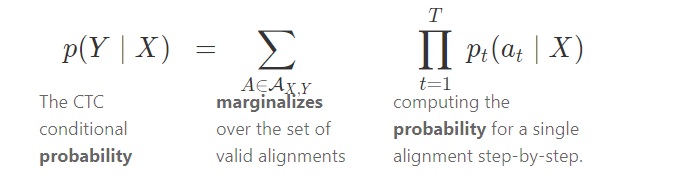
\includegraphics[width=0.5\textwidth]{img1.jpg}
        \caption{Mathematical Interpretation of Misfortune}
    \end{figure}
\end{itemize}

\subsection{\textbf{Architecture}}
Basically, 3 steps are involved :
\begin{itemize}
    \item Multi-scale feature Extraction : using  CNN(Convolutional Neural Network) layers used : 7 Layers
    \item Labeling the Sequence (BLSTM-CTC) : RNN layers used : 2 layers of LSTM with Connectionist temporal classification.
    \item Transcription : RNN output is decoded.
    \begin{figure}[h]
        \centering
        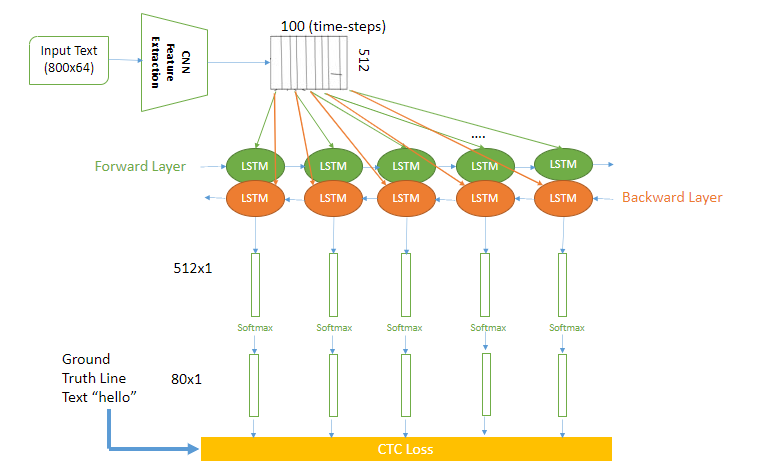
\includegraphics[width=0.5\textwidth]{img2.jpg}
        \caption{Network Architecture of implemented model}
    \end{figure}
\end{itemize}
\textbf{\\}
\textbf{CNN Layers}
\begin{itemize}
    \item The input image is given into the CNN layers.
    \item These layers are trained to extract the important features from the image.
    \item The proposed part consists of:
    \begin{itemize}
        \item Convolutional Layers
        \item RELU Activation Layer
        \item Max-Pooling Layer
    \end{itemize}
\end{itemize}
\textbf{}\\
\textbf{RNN Layers}
\begin{itemize}
    \item The output of CNN Layers is fed to RNN layers as input.
    \item We have decided to use RNN because it is excellent in sequence dependency and time-sequence operations.
    \item We have decided to use BLSTM implementation of LSTM, which in turn is an implementation of RNN.
    \item The output of CNN before it's FC-Layer is fed as input to the RNN. It is of form \textbf{(512x100)}.
    \item The constructed RNN will yield an output of form, \textbf{(100X80)}, i.e., 100 timesteps and 80 characters including blank.
\end{itemize}
\textbf{}\\
\textbf{Connectionist Temporal Classification Layer(CTC) Layer:}
\begin{itemize}
    \item While training, the CTC Layer is fed with output generated by RNN Layers as input.
    \item It will also be provided with ground truth text to calculate loss.
    \item During inferring, the Connectionist temporal classification is provided with the matrix and output the result by decoding the matrix.
    \begin{figure}[h]
        \centering
        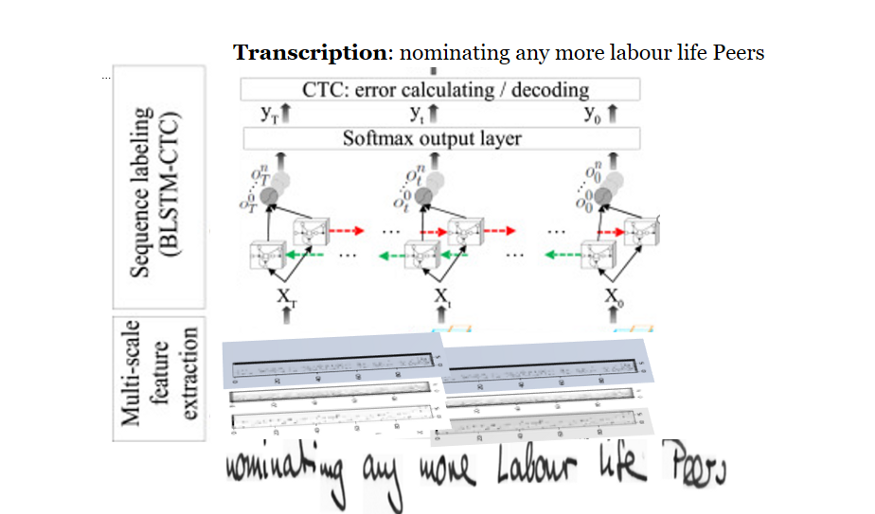
\includegraphics[width=0.5\textwidth]{img3.jpg}
        \caption{Transcript decoding process}
    \end{figure}
\end{itemize}

\textbf{\\}
\section{\textbf{Techniques Used}}
\subsection{\textbf{Convolutional Neural Network (ConvNet or CNN)}}
It is an extraordinary sort of Neural Network utilized successfully for picture acknowledgment and classification. They are exceptionally capable in territories like division/segmentation, object location, and acknowledgment, recovery, characterization, and so on, aside from creating vision in self-driving vehicles and robots as well.

\subsection{\textbf{Recurrent neural network (RNN)}}
It is a section of artificial neural networks where associations between trees structure a coordinated chart along a fleeting succession. This permits it to show fleeting dynamic behaviour. Gotten from feedforward neural organizations, RNNs can utilize their inward state (memory) to deal with variable length successions of data sources. This makes them appropriate to undertakings like unsegmented, associated penmanship acknowledgment or discourse acknowledgment.

\subsection{\textbf{Long short-term memory (LSTM)}}
It is an artificial RNN design. Unlike standard feedforward neural associations, LSTM has analysis affiliations. It can not just cycle single information focuses (like pictures), yet in addition whole arrangements of information (like speech, picture, video). For instance, LSTM is relevant to undertakings like unsegmented, associated penmanship acknowledgement, discourse acknowledgment and oddity recognition in network traffic or IDSs (interruption location frameworks).

\subsection{\textbf{Connectionist temporal classification (CTC)}}
It is a kind of neural network yield and related scoring capacity, for preparing recurrent neural networks (RNNs, for example, LSTM organizations to handle arrangement issues where t//he timing is variable. It tends to be utilized for errands like on-line penmanship acknowledgment or perceiving phonemes in discourse sound.

\textbf{\\}
\section{\textbf{DATASET}}
The IAM dataset is a combination of 13,353 images of handwritten lines of text written by 657 writers. The texts those writers transcribed are from the Lancaster-Oslo/Bergen(collection of english texts) Corpus of British English. It includes donatives from 657 writers making it a total of 1,539 handwritten pages containing 115,320 words and is designated as part of modern collection.  The dataset is labeled at various possible levels like at sentence, line, and word levels.

The dataset is freely available at fki site.[11] The database contains forms of ungoverned handwritten text, all of which were scanned at a resolution of 300dpi and saved in the format of PNG images with 256 gray levels. The images below provide samples of a complete form, a text line and some extracted words.\\
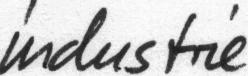
\includegraphics[width=0.27\textwidth]{img5.jpg} 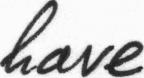
\includegraphics[width=0.18\textwidth]{img6.jpg}
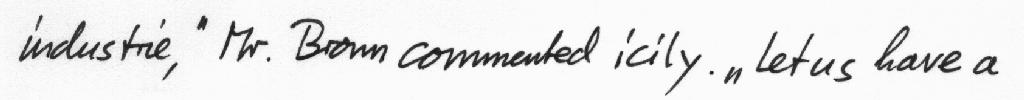
\includegraphics[width=0.5\textwidth, height=1.5cm]{img4.jpg}
\begin{center}
    Fig. 4: Sample images from IAM Dataset
\end{center}

The dataset was first distributed at the ICDAR 1999. Utilizing this dataset a HMM based acknowledgment framework for handwritten sentences was created and distributed at the ICPR 2000. The division conspire utilized in the second form of the information base is archived in and has been distributed in the ICPR 2002. The IAM-database released in October 2002 is the most latest.

\section{\textbf{ACTIVITY SCHEDULE}}
\textbf{\\}
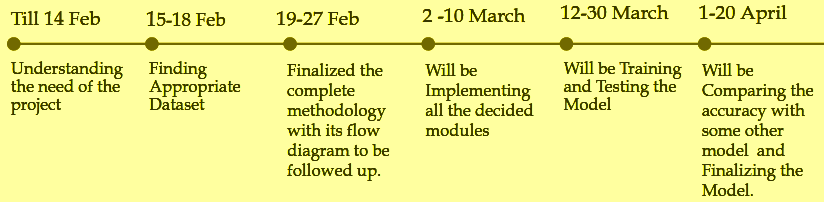
\includegraphics[width=0.45\textwidth, height=4cm]{img7.jpg}
\begin{center}
    Fig. 5: Activity Time Schedule
\end{center}

\section{\textbf{TOOLS USED}}
We have decided to use \textbf{PYTHON-3} for the implementation purpose of the project. It is commonly used Deep Learning projects and fairly easy to download and work upon. Additionally, it has a large user community so any problem or error will be easier to be dealt with. Also, it provided packages for every task whatsoever. We have decided to use following python packages, namely,
\begin{itemize}
    \item Numpy
    \item Flask
    \item Opencv-3
    \item Spell Checker \textbf{autocorrect} >= 0.3.0
    \item Tensorflow 1.8.0
\end{itemize}

\section{\textbf{RESULTS}}
\begin{itemize}
    \item We have trained the developed program\textbackslash model on IAM line image dataset which can be downloaded from the official repository. We have used 3000 images for training purposes.
    \item We have tested the developed program\textbackslash model. We have used 1000 images for testing purposes.
    \item We have observed train accuracy of 88\%.
    \item We have observed test accuracy of 81\%.
    \item We have used Levenshtein Distance as a metric to calculate accuracy. Levenshtein Distance finds sum of minimum number of operations (replace, delete, insert) required to transform obtained character sequence to given transcript.
    \item Figure 6 shows the output obtained for 2 testcases.
\end{itemize}
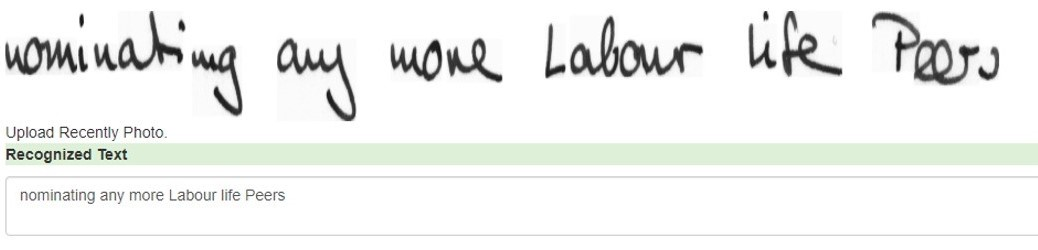
\includegraphics[width=0.45\textwidth, height=3cm]{img8.jpg}
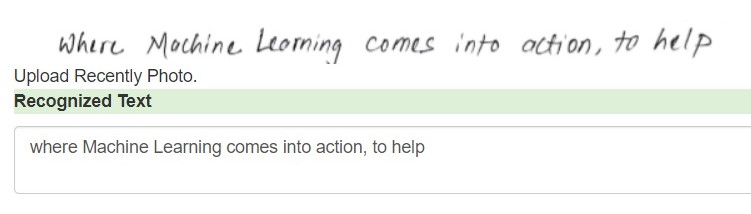
\includegraphics[width=0.45\textwidth, height=3cm]{img9.jpg}
\begin{center}
    Fig. 6: Outputs received for some input images
\end{center}

\section{\textbf{WORK DONE SO FAR}}
As of now, we have:
\begin{itemize}
    \item Understand about problem statement.
    \item Done with Literature survey with almost 3 papers including Base paper.
    \item Finalized the complete methodology with its flow diagram to be followed up.
    \item Implemented the modules that have to be made.
    \item Trained the model on Dataset.
    \item Tested the model with the input image.
\end{itemize}

\section{\textbf{REMAINING WORK}}
\begin{itemize}
    \item Compare the accuracy with some other model.
    \item Finally concluding everything from comparison to methodology.
    \item Optimizing the accuracy.
\end{itemize}

\section{\textbf{CONCLUSION}}
In this project, we have tried to recognize many address blocks written in capital/small letters. The strength of algorithms that we have used is that it is even able to recognize blocks/sentences in which the letters are slightly joined.

We have talked about how CRNN (CNN + LSTM) can perceive text in pictures with its itemized design. The model comprises of 7 CNN and 2 LSTM layers and yields a character-likelihood grid. We have used Convolutional Recurrent Neural Network to recognize the Handwritten line text image without pre-segmentation into words or characters. Then use CTC loss Function is used to train.

The model has yielded an accuracy of \textbf{88\%} on training, on testing the received accuracy is \textbf{81\%}. We have used Levenshtein Distance as a metric to determine the accuracy of the model.

\section{\textbf{References}}
[1] Plamondon, Réjean, and Sargur N. Srihari. "Online and offline handwriting recognition: a comprehensive survey." Pattern Analysis and Machine Intelligence, IEEE Transactions on 22.1 (2000): 63-84.

[2] Liu, Xia, and Zhixin Shi. "A format-driven handwritten word recognition system."2013 12th International Conference on Document Analysis and Recognition. Vol. 2. IEEE Computer Society, 2003

[3] Park, Jaehwa, Venu Govindaraju, and Sargur N. Srihari. "OCR in a hierarchical feature space." Pattern Analysis and Machine Intelligence, IEEE Transactions on 22.4 (2000): 400-407.

[4] Singh, Sameer, Mark Hewitt,“Cursive Digit And Character Recognition on Cedar Database”, Pattern Recognition, 2000.Proceedings. 15th international conference on. Vol. 2. IEEE 2000.

[5] Graves and N. Jaitly, “Towards end-to-end speech recognition with recurrent neural networks,” in Proceedings of the 31st International Conference on Machine Learning, 2014, pp. 1764–1772.

[6]  U. Marti and H. Bunke, “The IAM-database: an English sentence database for offline handwriting recognition,” International Journal on
Document Analysis and Recognition, vol. 5, no. 1, pp. 39–46, 2002.

[7]  B. Shi, X. Bai, and C. Yao, “An End-to-End Trainable Neural Network for Image-based Sequence Recognition and its Application to Scene
Text Recognition,” IEEE Transactions on Pattern Analysis and Machine Intelligence, vol. 39, no. 4, pp. 2298–2304, 2016.

[8]  E. Kavallieratou, K. Sgarbas, N. Fakotakis and G. Kokkinakis, “Handwritten Word Recognition based on Structural Characteristics and Lexical Support”, by Wire Communications Lab, University of Patras, 26500 Patras, 2003.

[9] Paul D. Gader, Magdi Mohamed, and Jung-Hsien Chiang, “Handwritten Word Recognition with Character and Inter-Character Neural Networks”, 2012

[10] Shushant Chak, Ambalika Sharma, “HandWritten Character Recognition using Artificial Neural Network” by Indian Institute of Technology Roorkee, Uttarakhand, India.

[11] https://fki.tic.heia-fr.ch/databases/iam-handwriting-database

\end{document}